\section{Optimizing the aTag Enhancements}
We have specified several improvements to our encoding scheme. We will not present methods for optimizing the memory usage and width of the scheme.

\subsection{Width with Variable Length Identifiers}
We discussed the used of prefix codes to take advantage of the variable amount of space available for superset identifiers. We can determine the optimal width possible from using a prefix free code with Kraft's Inequality. Kraft's inequality states that, given a requirement of $N$ codewords where each codeword has a limited width of $L_i$, then it is possible to construct a prefix code if the following equation is satisfied:
$$ \sum_{i = 0}^{N}{2^{-L_i} \le 1} $$
Where $width_i$ is the maximum width available for the $i^{th}$ superset's identifying codeword. We can use this inequality to determine the smallest tag width possible, denoted by $W_{min}$, for a given list of supersets. Note that, for the $i^{th}$ superset, the space available for the identifying codeword will be $L_i = W_{min} - |superset_i|$. Using this, we can solve for $W_{min}$.\\

\begin{equation} \label{eq1}
 \begin{split}
  \sum_{i = 0}^{N}{2^{-(W_{min} - |superset_i|)}}   \le  1 \\
  \implies 2^{-W_{min}} \sum_{i = 0}^{N}{2^{|superset_i|}}   \le  1 \\
  \implies  \sum_{i = 0}^{N}{2^{|superset_i|}}   \le  2^{W_{min}} \\
 \implies   \lceil\log_2{\sum_{i = 0}^{N}{2^{|superset_i|}}}\rceil  =  W_{min}
\end{split}
 \end{equation}
 
 The left hand side is straightforward to solve, giving us the minimum width possible for the input list of supersets. We can then use this value to find each $width_i$, or the width available for the identifier of the $i^{th}$ superset.
 
 Once all the identifier widths are known, finding an actual prefix code can be accomplished by building a binary code tree. Figure \ref{fig:variable_id}(c) shows such a code tree. Each node $n$ in the tree is associated with a binary string $s$. The left child of $n$ will have string $s + '0'$, and the right child will have $s + '1'$. The root of the tree corresponds to the empty string. A consequence of this is that node in the tree is a prefix of all of its children. To construct a prefix code, only leaf nodes may be codewords. 
 
 The code is built with a level-by-level tree construction. We begin with level 0, the root node. Two children are added to the root to create level 1, corresponding to strings $'0'$ and $'1'$, the length 1 binary strings. The construction proceeds as follows:  After creating the $k^th$ level of the tree, if there exists an $i$ such that $width_i = k$, we assign an arbitrary node in the current level to be the $i^th$ codeword. After all such codewords are assigned, the next level is constructed. Child node are added for each node in the current level that was not assigned as a codeword, and the construction proceeds until all codewords are assigned.
 
\subsubsection{Minimizing Kraft to Decrease Tag Width}
We've shown how to find a prefix code which optimally minimizes the tag width for a fixed list of supersets, but the problem becomes more interesting if we are permitted to modify the list of supersets. 

Recall that the tag width $W_min$ for a list of supersets is given by the equation $W_{min} = \lceil\log_2{\sum_{i = 0}^{N}{2^{|superset_i|}}}\rceil$. If we can reduce the sum within the log term, we may be able to decrease the width. This can be done with a simple greedy algorithm. Consider every pair of supersets. Find the pair which, when removed and replaced by their union, maximally decreases the sum ${\sum_{i = 0}^{N}{2^{|superset_i|}}}$. If no union decreases the sum, instead choose the union that minimally increases it. If this union operation increases $W_min$, stop. Otherwise, perform the union and then repeat. 

\subsection{Partial to Total Ordering}
The encoding scheme is primarily used for encoding unordered sets of attributes, but some applications may have orderings. For the case of service chaining, it may not make sense to visit network middleboxes in an arbitrary order. 
Unfortunately, converting a partially ordered universe to a totally ordered universe is not straightforward. There can potentially be sets of incomparable elements, rather than just pairs, making it unclear which elements to split to resolve incomparabilities with the least number of additional bits. In the worst case where every pair of elements is incomparable, 

 Figure \ref{fig:ordering} shows one algorithm for doing so at a high level. For a concrete example, we are given four input sequences we wish to encode, shown in \ref{fig:ordering}(a). We assume that these sequences \textit{almost} follow an underlying ordering, but that there are a few incomparable sets of elements. In this example, $B$ is incomparable with $C$ because $B$ appears both before and after $C$. 

To systematically identify these incomparable elements, we construct the sequence graph, shown in \ref{fig:ordering}(b). In the sequence graph, element $u$'s node has an edge to element $v$'s node if $u$ appears before $v$ in any sequence. We then run an algorithm for finding Strongly Connected Components (SCCs) on this graph. A strongly connected component is a set of nodes such that for every pair of nodes $u$ and $v$ in the set, $u$ has a path to $v$ and vice versa. In this context, every SCC corresponds to a set of incomparable elements. Figure \ref{fig:conflict_res} shows the process for determining which elements to split to create a new, totally ordered universe. Figure \ref{fig:ordering}(d) and (e) shows the result of using this new ordering to modify each sequence. 


\begin{figure}[t!] 
\begin{minipage}{1\linewidth}
\begin{subfigure}[c]{0.96\linewidth}
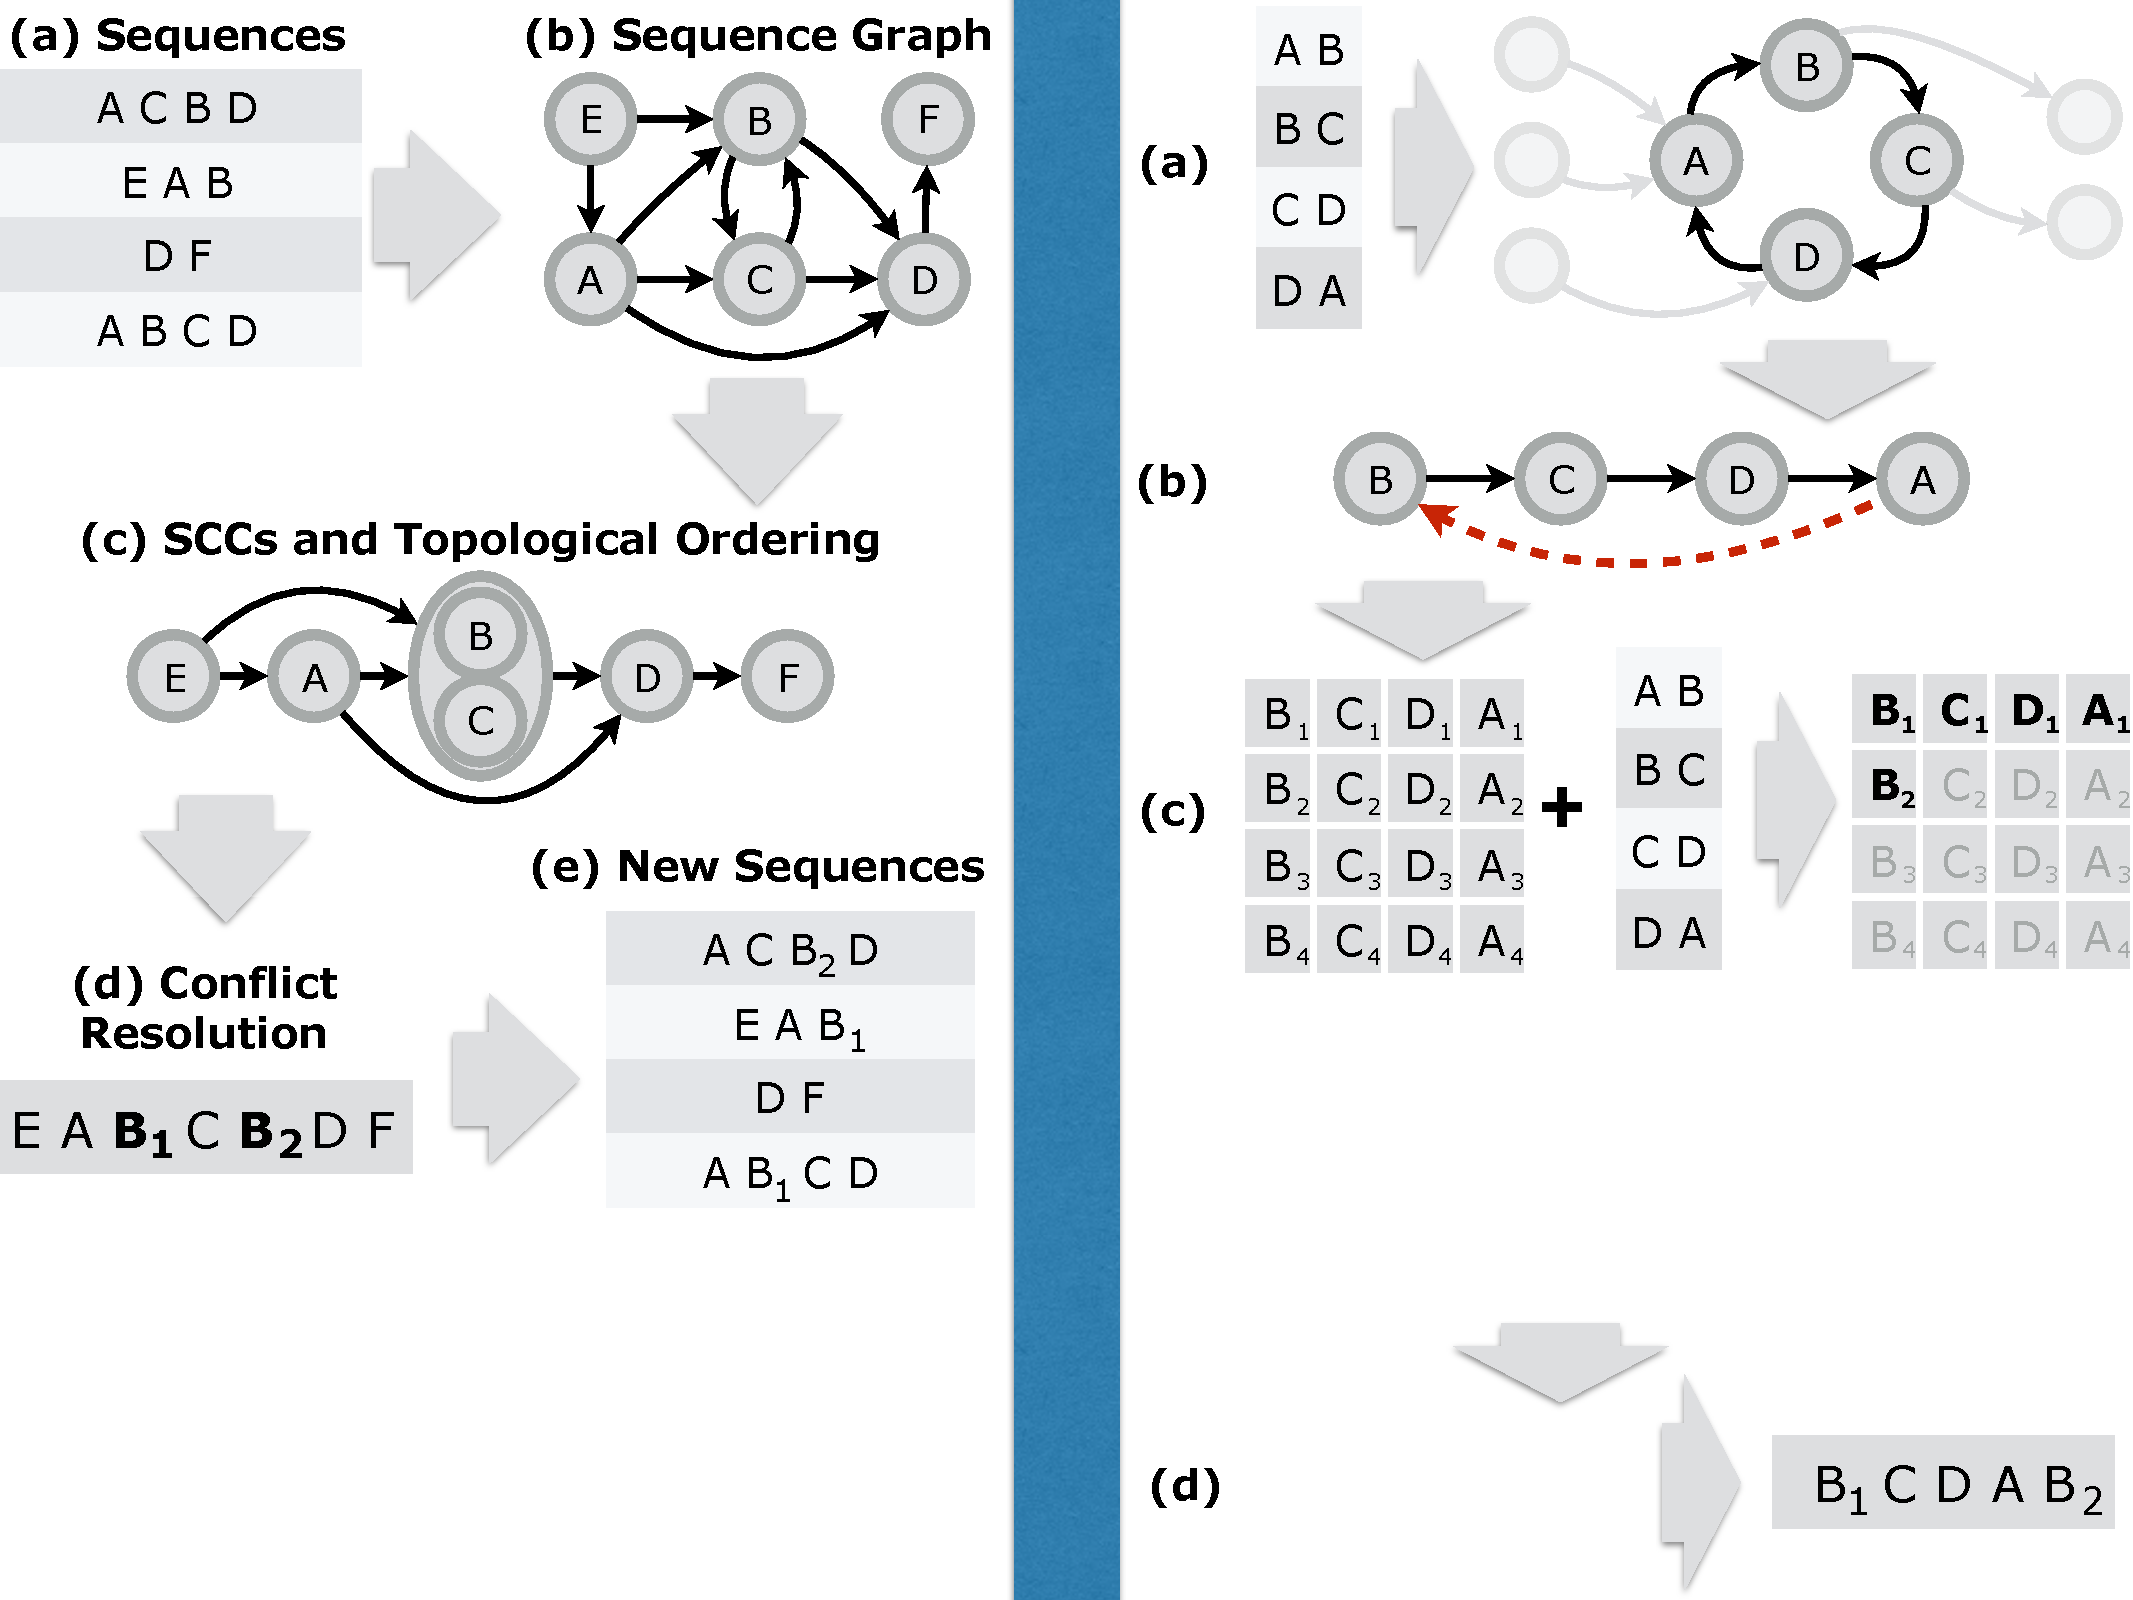
\includegraphics[trim={0 6cm 19.2cm 0}, clip, width=\linewidth]{figures/partial_ordering}
\end{subfigure} 
\end{minipage} 
\caption{This figure shows, at a high level, the process for converting a partial ordering to a total ordering by identifying incomparable elements and creating duplicates to resolve the incomparabilities. (a) shows the four input ordered sequences. In (b), we create a graph of the elements, where there is an edge from $u$ to $v$ if $u$ appears before $v$ in some sequence. (b) shows how the graph can be broken up into an ordered Directed Acyclic Graph (DAG) of Strongly Connected Components (SCC), where each SCC corresponds to a set of incomparable elements. (d) shows the result of splitting elements to resolve incomparability, which is covered in more depth in figure \ref{fig:conflict_res}. In (e), the original sequences are modified with the splits such that each sequence adheres to a total ordering.}
\label{fig:ordering}
\end{figure}



\begin{figure}[t!] 
\begin{minipage}{1\linewidth}
\begin{subfigure}[c]{0.96\linewidth}
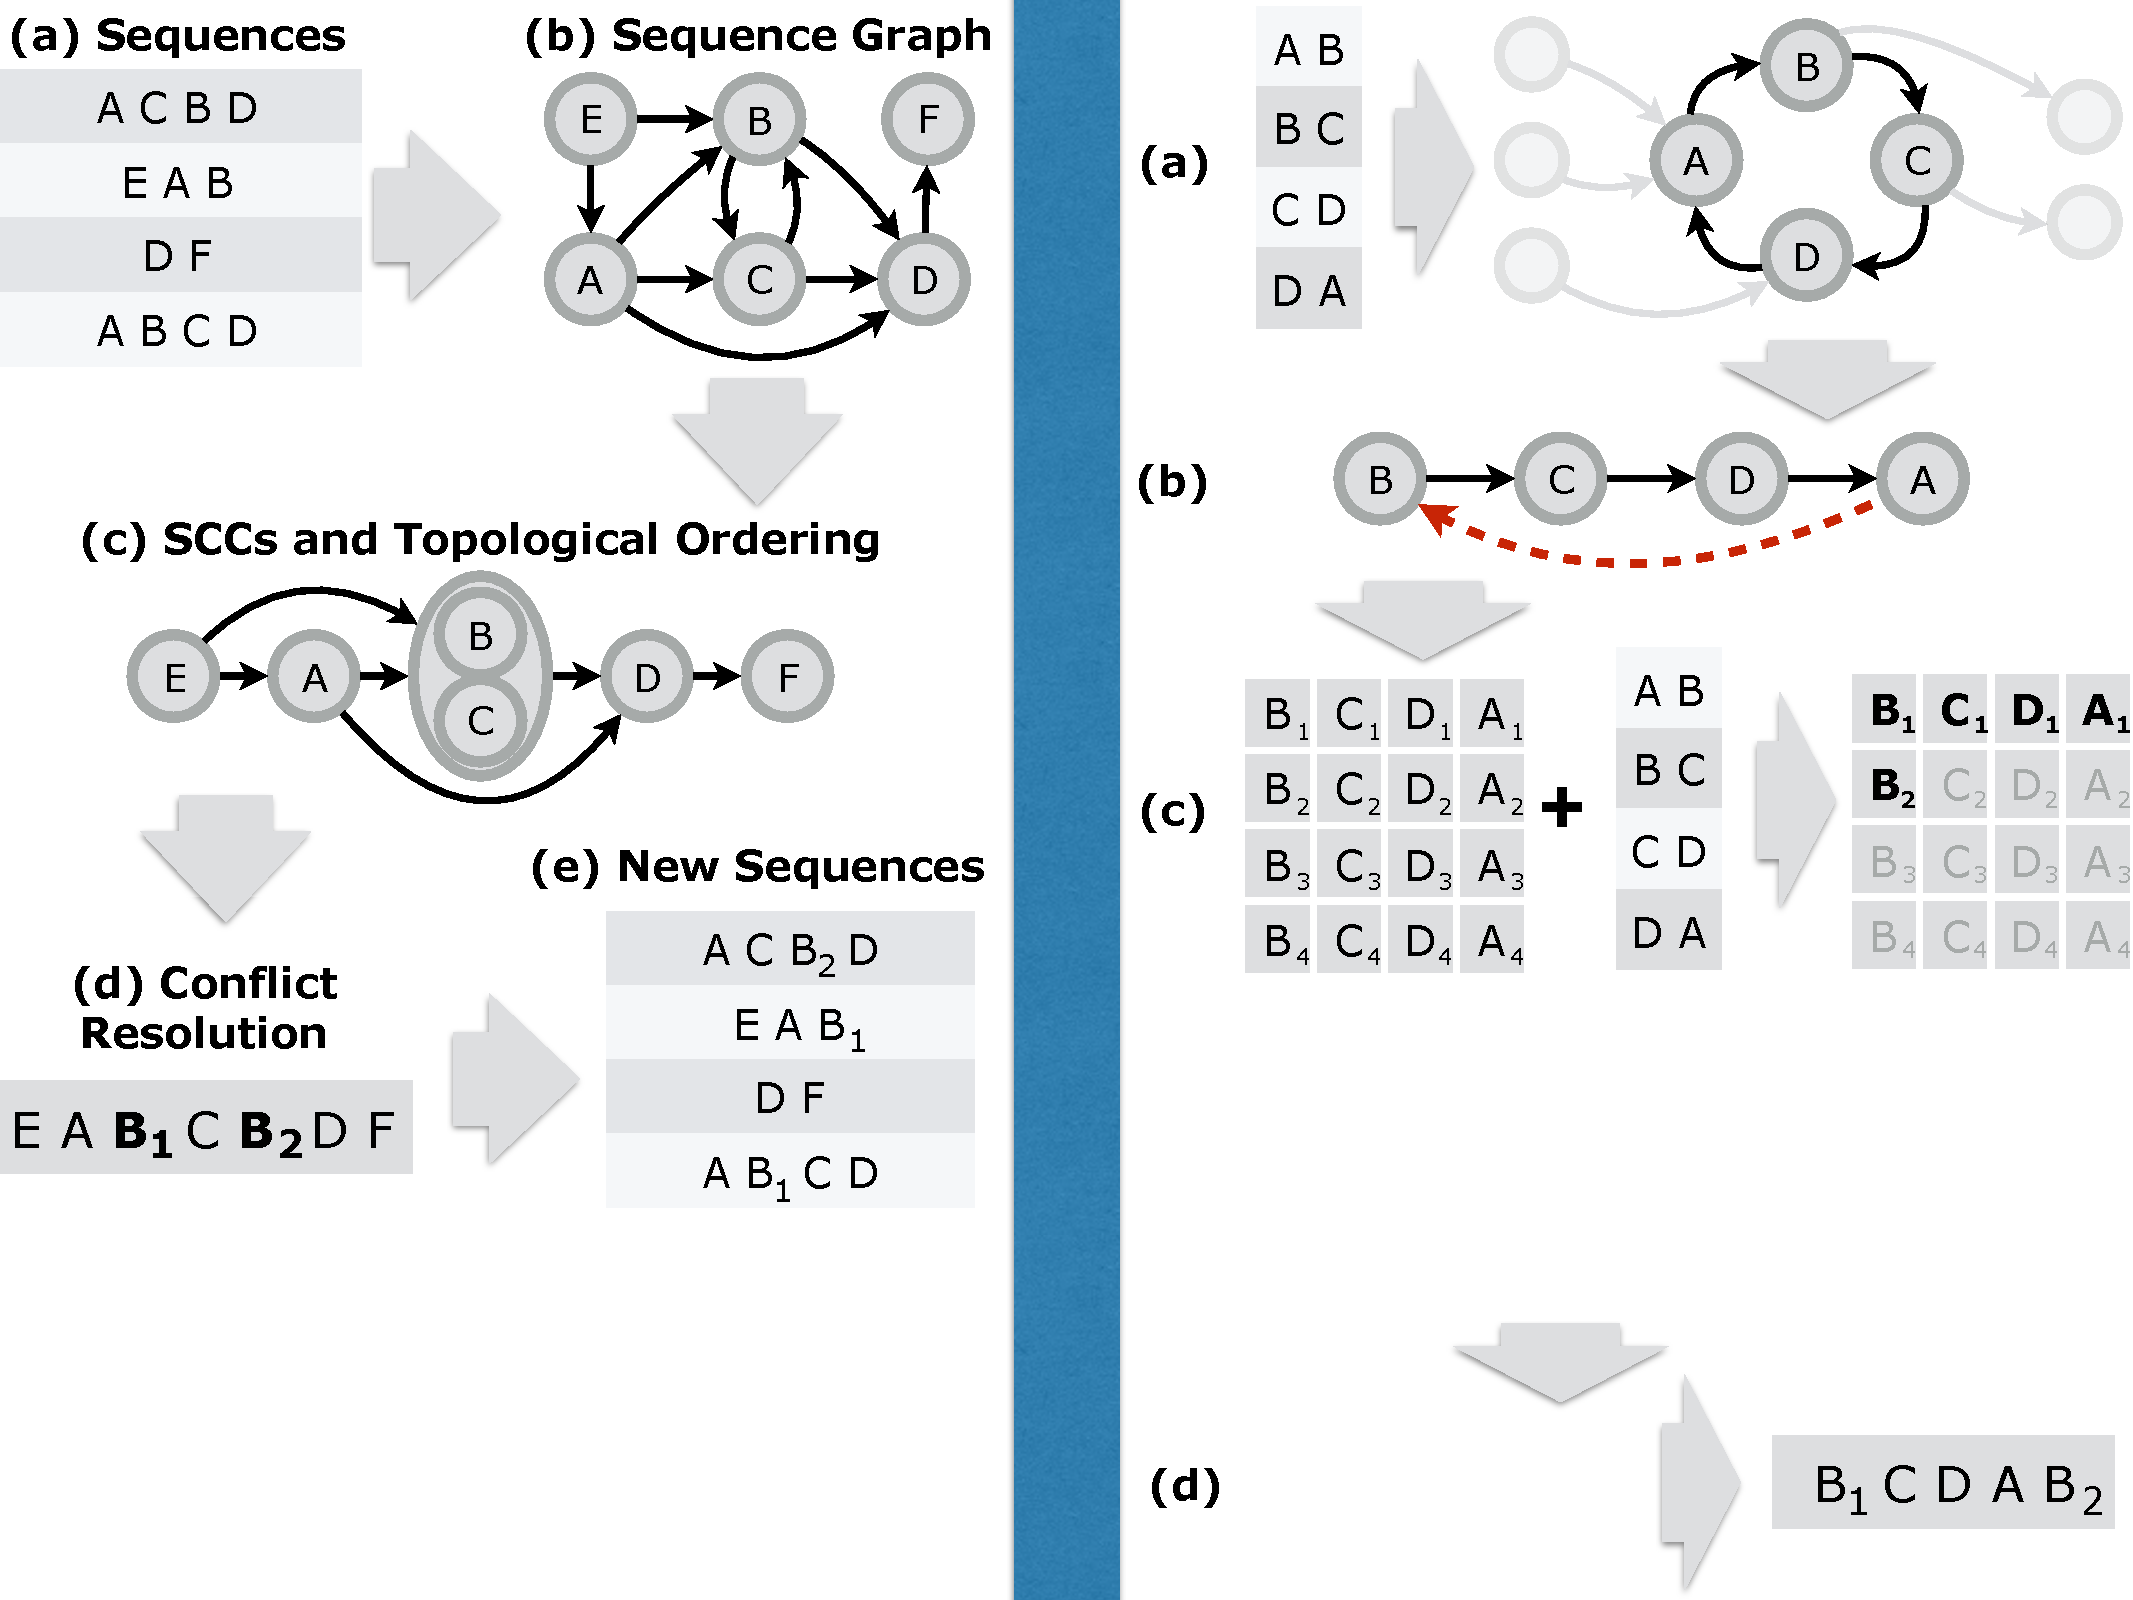
\includegraphics[trim={19.2cm 10cm 0 0}, clip, width=\linewidth]{figures/partial_ordering}
\end{subfigure} 
\end{minipage} 
\caption{This details the Conflict Resolution step of the algorithm. (a) shows a SCC corresponding to four incomparable elements. (b) shows an 'almost' ordering of the SCC nodes, which minimizes the number of backward edges. (c) shows how the almost ordering is used to construct a worst-case quadratically-sized universe, which is then traversed by every sequence to determine which splits are necessary. }
\label{fig:conflict_res}
\end{figure}